\subsubsection{Есть ли ОС в дифференциальном усилителе, и если есть, то какие они и чем определяются?}

\begin{center}
	\begin{figure}[h!]
		\center{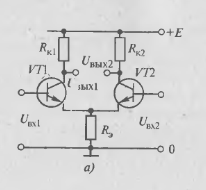
\includegraphics[scale=0.9]{DiffUs}}
		\caption{Схема}
	\end{figure}
\end{center} 
ДУ отличает высокая стабильность работы, малый дрейф нуля, большой коэффициент усиления дифференциального сигнала и большой коэффициент подавления синфазных помех.
Любой ДУ выполняется по принципу сбалансированного полностью симметричного моста ($R_{k_1} = R_{k_2}$ все параметры транзисторов совпадают).. 

При анализе работы ДУ принято выделять в нем два плеча, одно из которых состоит из транзистора VТ1 и резистора Rк1, второе  — из транзистора VТ2 и резистора Rк2. Каждое плечо ДУ является каскадом ОЭ. Таким образом, можно заключить, что в состав ДУ входят два каскада ОЭ. В общую цепь эмиттеров транзисторов также включен резистор $R_e$. Для корректной работы ДУ необходимо выполнить 2 условия: сделать плечи каскада симметричными (для обеспечения одинаковой реакции на одинаковые воздействия и для избежания дрейфа нуля) и обеспечить наличие ООС для еще большего уменьшения коэффициента усиления синфазного сигнала.

*Синфазные сигналы  - сигналы с равными амплитудами, формами и фазами. $U_{in_1} = U_{in} +- \Delta U$ ; $U_{in_2} = U_{in} +- \Delta U$. Изменение температуры, паразитные наводки, старение элементов и др. можно рассматривать как синфазные входные воздействия => нужно их подавлять, они вредны для работы любого усилителя.

Как раз таки резистор $R_e$ обеспечивает последовательную ООС по току. Рассмотрим симфазное воздействие: Пусть на оба входа пришло положительное воздействие. Тогда токи через транзисторы увеличатся, => увеличится ток через $R_e$ \Rightarrow $U_{R_e} \uparrow$ => увеличится потенциал в эмиттере => транзисторы подзапрутся. Коэффициент усиления синфазного сигнала имеет вид:

$$
K_{s/f} = -\frac{\alpha R_k}{2R_e}
$$

Видно, что выгодно ставить как можно больший резистор $R_e$, но с увеличением $R_e$ приходится сталкиваться с проблемой обеспечения необходимого режима работы транзисторов по постоянному току. Т.е. приходится увеличивать для данных $I_{K1}$; $I_{K2}$ питание $E_p$. Это неразумно, поэтому часто ставят вместо резистора ГСТ, выполненный, как правило, на транзисторе.

Если же мы имеем дело с парафазным сигналом, то приращения $\Delta U_{in}$ и $-\Delta U_{in}$ вызовут противоположные приращения токов в плечах, и результирующий ток через резистор $R_e$, а значит, и напряжение на нём не изменится. Таким образом, ООС играет роль только для синфазного сигнала. 
